% Unified working manuscript; no submission or editorial decision is implied.
% Existing frozen manuscripts, methods, and result fragments remain unchanged.
\documentclass[sigconf,nonacm]{acmart}
\usepackage{pvldb}
\renewcommand\vldbdoi{XX.XX/XXX.XX}
\renewcommand\vldbpages{XXX-XXX}
\renewcommand\vldbavailabilityurl{https://github.com/mandu5/sparse-vus/tree/research/pvldb-20261024}
\newtheorem{theorem}{Theorem}
\newtheorem{lemma}{Lemma}
\newtheorem{proposition}{Proposition}
\newtheorem{corollary}{Corollary}
\newcommand{\ind}{\mathbf{1}}
\newcommand{\TP}{\mathrm{TP}}
\newcommand{\TPR}{\mathrm{TPR}}
\newcommand{\FPR}{\mathrm{FPR}}
\emergencystretch=2em
\begin{document}
\title{Exact VUS Evaluation by Support Events and Shared Interval Geometry}
\author{Youngmin Ko}
\email{rhdudals0505@naver.com}
\affiliation{\institution{Independent Researcher}\country{Republic of Korea}}
\begin{abstract}
Volume Under the Surface (VUS) evaluates anomaly scores across thresholds and temporal tolerance widths. We derive an exact support-event representation for the original dynamic VUS operator. Thresholds with no active support have zero precision--recall contribution; their receiver-operating-characteristic contribution requires a predecessor correction. Complete global ties and merged anomaly components remain explicit. Standard fixed-width ranking and two-distance interval geometry give $O(n+(L+1)Q)$ evaluation, where $Q$ is maximum-buffer support. Shared-label preparation further reduces repeated work across score columns. A prospectively fixed study uses 73 complete real series from three public collections and eight fixed detector procedures, producing 584 unrounded score vectors per host. Fresh execution on Apple M1 Pro and AMD EPYC preserves the main result: directly timed collection workflows are $16.2$--$23.0\times$ faster than an unchanged exhaustive PR comparator. Matched ROC+PR workflows improve by $22.4$--$42.5\times$ over a public cumulative-sum implementation. Compiled controls distinguish compression, implementation and sharing effects: an optimized conventional direct-ramp control is faster than our single-model implementation at the primary width, while batch evaluation improves over it. Exact evaluation also dominates the measured 250-threshold approximation in both latency and numerical fidelity on this workload. A public nine-metric consumer illustrates the scope limit: its VUS stage improves $66.1\times$, but total latency only $1.031\times$ because other metrics dominate. We report paired uncertainty, shared-label dependence, unfavorable regimes and process-memory costs. Mathematical exactness and measured floating-point parity are distinct guarantees.
\end{abstract}
\maketitle
\vldbtopmatter
\section{Introduction}
Evaluation is a repeated data-analysis operation in time-series anomaly
benchmarks: stored score vectors from several detectors or configurations are
joined with the same labels, evaluated, and compared to select a numerical
winner. Volume Under the Surface (VUS) aggregates range-aware precision--recall
(PR) or receiver-operating-characteristic (ROC) integrals over temporal
widths~\cite{paparrizos2022,boniol2025}. Exhaustive evaluation integrates every
complete distinct-score threshold at every integer width. Sampling thresholds
reduces work but changes the returned scalar and can change the selected model.
The computational question is whether the exact operator needs all those states.

Substantial acceleration already exists. Boniol et al. separate
maximum-buffer support from unaffected regions and reuse static work.
Klein's fast-VUS uses support-score cumulative sums; Benchopt uses dense
cumulative sums and segment maxima~\cite{boniol2025,klein2026,benchopt2026}.
However, reusing support statistics still leaves a second question: which
threshold states must be retained to compute the scalar integral? PR and ROC
give different answers, because a threshold with no new true-positive mass
can still contribute ROC area.

We derive a scalar event representation of the original dynamic operator.
Inactive threshold runs have zero PR area, and their ROC area is a horizontal
rectangle preceding the next active transition. This distinction matters:
connecting only retained ROC endpoints gives an incorrect answer, even without
buffers. Complete global score ties must include predictions outside support,
and expanded anomaly components must merge under the target's overlap rule.
A two-distance lemma removes repeated interval-ramp construction. With standard
binary64 radix preparation, exhaustive evaluation takes
$O(n+(L+1)Q)$, where $n$ is series length, $L$ is maximum width, and $Q$ is
maximum-width support. This is a support-sensitive bound, not a claim that
sorting arbitrary real numbers is linear.

The data-management contribution is an exact implementation of a recurring
analytics operator on stored detector profiles. It reduces the states and
width-dependent work needed for the same aggregate, and exposes shared-label
preparation when several score columns are evaluated together. The latter uses
standard caching and loop interchange; its value is measured separately from
the event representation. Our complete workflow reads stored arrays, evaluates
all score columns, selects winners, and writes the decision table. We do not
claim a new detector, deployment selector, metric, or database execution engine.

A preliminary evaluator and working manuscript were publicly released as
Sparse VUS 0.3.0 on 21 October 2026~\cite{sparsevus03}. This paper presents the
complete exact-evaluator work and separately measures the sharing increment
over that unrefereed software precursor.

The paper makes three connected contributions. First, it proves the
support-event identities and their complexity, including the dynamic
denominator, complete ties, and ROC predecessor correction. Second, it gives
an implementation and preparation/streaming ablations for repeated evaluation
with a shared label sequence. Third, it evaluates full public calls and complete
collection workflows on a prospectively frozen, full-precision panel, followed
by a separately frozen strongest-comparator and approximation study. The
experiments report confidence intervals, label-block sensitivity, exact-value
checks and unsuccessful alternatives. The primary study uses three public
univariate collections and eight fixed score-generation procedures, with fresh
execution on two CPU architectures. Record reuse and the scope of warm
stored-score evaluation are stated with the experimental protocol.
\section{Target and exact event representation}
Let $y\in\{0,1\}^n$ contain both classes and $s\in\mathbb{R}^n$ contain finite
scores after binary64 conversion. Larger scores indicate greater anomaly
evidence. Let $P_0=\sum_i y_i$, and let the $K$ maximal original anomaly
intervals have inclusive endpoints $[a_k,b_k]$ in temporal order. Widths are
the integers $w=0,\ldots,L$. The continuous label $a_i^{(w)}$ is one on
original positives. An interval contributes $\sqrt{1-d/w}$ outside its
endpoints at integer distance $1\le d\le\lfloor w/2\rfloor$; contributions
are summed and clipped at one. At $w=0$ no ramp is added. Expanded intervals
that overlap merge, while adjacent nonoverlapping intervals remain separate.
This is the original dynamic VUS target pinned to the official
\texttt{RangeAUC\_volume\_opt} source at revision
\texttt{467bace0}, configured for exhaustive thresholds~\cite{vusreference}.
It is not shared by all software named VUS.

For a threshold $t$, define
\begin{align}
 p_i(t)&=\ind\{s_i\ge t\}, & C(t)&=\sum_i p_i(t),\\
 A(t)&=\sum_i y_i p_i(t), &
 B(t)&=\sum_i(1-y_i)a_i^{(w)}p_i(t),\\
 T(t)&=A(t)+B(t), & P(t)&=P_0+B(t)/2,\\
 N(t)&=n-P(t).
\end{align}
Let $H(t)$ count expanded components hit by at least one predicted positive,
and let $K_w$ count those components. The curve coordinates are
\begin{align}
 R(t)&=\min\{T(t)/P(t),1\}\,H(t)/K_w,\\
 F(t)&=(C(t)-T(t))/N(t), & \pi(t)&=T(t)/C(t).
\end{align}
Precision is used only at nonempty retained thresholds, where $C(t)>0$;
the initial origin requires no precision value.
The denominator is positive: $P(t)\le(n+P_0)/2<n$. ROC integrates trapezoids
from the origin through complete distinct descending score thresholds to
the explicit terminal $(1,1)$. PR uses the right-step sum
$\sum_j(R_j-R_{j-1})\pi_j$, with $R_0=0$. Each VUS scalar is the arithmetic
mean over every width. Signed horizontal ROC increments are preserved; the
derivation does not replace a dynamic denominator by a fixed one.

Let $S_w=\{i:a_i^{(w)}>0\}$, $Q_w=|S_w|$, and $Q=Q_L$. For an active event
with score $v_j$, precompute the complete global counts
$c_j^>=|\{i:s_i>v_j\}|$ and $c_j^\ge=|\{i:s_i\ge v_j\}|$. They include
positions outside $S_w$ and outside $S_L$.

\begin{lemma}[Inactive threshold runs]
Between consecutive active score events at a fixed width, $T,B,P,N,H,R$
are constant. Omitted thresholds contribute a horizontal ROC rectangle and
zero PR area. At an active score, its complete global numerical tie is a
single transition.
\end{lemma}
\begin{proof}
A newly admitted inactive point has zero weight and cannot hit an expanded
component. Only $C$ changes. The horizontal increments
$(\Delta C)/N$ telescope at fixed height $R$. All positions tied with an
active event enter at its global threshold, so both counts must retain them.
\end{proof}

If the previous retained state is $(T_o,N_o,R_o,c_o)$, event $j$ contributes
\begin{align}
 f_j^-&=(c_j^>-T_o)/N_o,\\
 \Delta\mathrm{ROC}_j&=
 (c_j^>-c_o)R_o/N_o+(F_j-f_j^-)(R_j+R_o)/2,\\
 \Delta\mathrm{PR}_j&=(R_j-R_o)T_j/c_j^\ge.
\end{align}
The initial state is $(0,n-P_0,0,0)$, and afterwards $c_o=c_j^\ge$.
Connecting retained endpoints without the intervening rectangle is
incorrect. For example, $y=(1,0,1,0)$, $s=(3,2,1,0)$ and $L=0$ give ROC
area $0.625$; connecting support endpoints alone gives $0.8125$.

\begin{lemma}[Two-distance geometry]
The weight of a non-original point is determined by its distances $d_1,d_2$
to the nearest two distinct original intervals. It is zero if
$d_1>\lfloor w/2\rfloor$, one if $d_2\le\lfloor w/2\rfloor$, and
$\sqrt{1-d_1/w}$ otherwise.
\end{lemma}
\begin{proof}
Every active ramp has weight at least $1/\sqrt2$. Two contributions therefore
clip to one. If exactly one interval contributes, its distance determines
the weight. Distances to ordered intervals are monotone moving away on each
side, so two neighbors on each side contain the nearest two intervals.
\end{proof}

\begin{theorem}[Support-event evaluation]
\label{thm:support-events}
In a unit-cost model with score comparisons and metric arithmetic, including
square roots, both exhaustive scalar integrals can be computed in
$O(n\log(Q+1)+(L+1)Q)$ time and $O(n+Q)$ auxiliary words.
\end{theorem}
\begin{proof}
Extract original intervals and maximum support in $O(n)$ time. Sort the $Q$
support scores and group equal values. Binary-search all $n$ scores among
these groups to obtain complete global counts $c^>,c^\ge$ without sorting
off-support scores, at cost $O(n\log(Q+1))$. The ordered-interval geometry
can be prepared within this bound. At each width, compute support weights,
component membership, grouped masses and first component-hit events in
$O(Q+K)$ time. A scan of the at most $Q$ event groups integrates the
preceding rectangles, complete tied transitions and terminal ROC tail.
The inactive-run lemma makes this identical to the exhaustive target in
exact metric arithmetic. Stream the width mean using input-, support- and
interval-sized arrays. Since $K\le Q\le n$, the stated bounds follow.
\end{proof}

\begin{proposition}[Fixed-binary64 preparation]
\label{prop:radix}
For finite binary64 scores, complete global tie counts, the score ordering
of maximum support, and its two-distance geometry can be prepared in
$O(n+Q+K)$ time and $O(n+Q)$ auxiliary words. Discrete work uses a word-RAM
with input indices, counts, widths, and intermediate index arithmetic
fitting words. Metric arithmetic, including square roots, has unit cost.
\end{proposition}
\begin{proof}
Normalize signed zeros. Complement a negative score's bit pattern and flip
the sign bit of a nonnegative score, then complement the result to obtain a
descending numerical key. Eight stable byte-counting passes order these
64-bit keys in $O(n)$ time. Scan complete ties and retain their starting and
ending global ranks. Filter the permutation to maximum-support positions.
A temporal scan with a monotone interval pointer computes nearest distances
and owners in $O(Q+K)$ time. All arrays are input- or support-sized.
\end{proof}
Radix sorting and floating-point key transforms are established
techniques~\cite{demaine2011radix,herf2001radix}. This assumption does not give
linear sorting of arbitrary real scores or a bit-complexity bound for growing
precision. Conversion defines numerical ties, including collisions between
distinct large integer inputs.

The same support-event width kernel combined with this preparation gives
$O(n+(L+1)Q)$ time. This is the basic Sparse VUS evaluator; its improvement
over a dense rank sweep depends on $Q$, rather than recall saturation.
The released PR-only implementation retains $L+1$ scalar width results,
adding $O(L)$ words; streaming removes this storage. Input-sized ranking
arrays remain necessary in this construction, so the memory is not
support-only.

\section{Prior algorithms and comparison scope}
Boniol et al.'s optimized VUS algorithms retain threshold loops within
widths and support-region summation~\cite{boniol2025}. The official source
additionally creates full-length prediction and label arrays per threshold.
Klein removes repeated threshold-wise summation through support cumsums,
but still constructs maximum-support and full-length coverage arrays at
each width~\cite{klein2026}. Benchopt cumsums over all positions and computes
component-hit counts through segment maxima~\cite{benchopt2026}.
Table~\ref{tab:algorithm-scope} distinguishes these mechanisms from the
new reductions. Its costs describe inspected operations, not cross-library
runtime predictions.

\begin{table*}[t]
\centering\small
\setlength{\tabcolsep}{4pt}
\begin{tabular}{p{0.19\textwidth}p{0.29\textwidth}p{0.43\textwidth}}
\toprule
Construction & Threshold and width work & Semantic/comparison qualification\\
\midrule
Boniol Algorithms 2/3 & Per-width threshold loop; $Q$-support sums per threshold & Static-support reuse and cached predictions are prior techniques; the released target uses $\ge$ ties.\\
Klein fast-VUS & Per-width support cumsum, full-series coverage and threshold arrays & PR only; use $H=n$, not the sampled default $H=250$. Explicit arrays cost $\Omega(Q+n+H)$ per width.\\
Benchopt & Per-width full-series cumsum and threshold arrays & Computes both ROC and PR; $H=n$ covers exhaustive ties. Explicit arrays cost $\Omega(n+H)$ per width.\\
FF-VUS & Batched width/threshold matrices and support masking & Native linear/max ramps differ from the pinned target; public wrapper rounds scores; Torch has an existence approximation fallback.\\
Sparse support events & $O(n+(L+1)Q)$ with fixed-key preparation & Removes inactive thresholds while retaining global counts and exact ROC rectangles; no prefix stop is required.\\
\bottomrule
\end{tabular}
\caption{Algorithmic comparison. $H$ is the requested threshold count;
$Q$ is maximum support. External array-cost lower bounds omit
additional ramp, sorting and search work. Batched FF-VUS has no single
sequential per-width loop. Our bounds use the stated arithmetic model.}
\label{tab:algorithm-scope}
\end{table*}

Sorted sweeps, complete ties and trapezoids are established ROC
techniques~\cite{fawcett2006}. scikit-learn~1.0.2 explicitly truncates PR at
full recall after forming cumulative counts~\cite{sklearn102}. Therefore
full-recall stopping and zero-area PR suffixes are not new principles.
Our earlier artifact comparison includes last-original-positive stopping, which already
ensures saturation. The specific questions are whether buffer mass permits
an earlier stop and whether preparation avoids paying for the discarded
suffix. Reversible list updates~\cite{knuth2000}, union-find~\cite{tarjan1984},
radix ordering~\cite{demaine2011radix,herf2001radix} and exact
accumulators~\cite{neal2015} are established tools used in the construction.

Sylligardos reports preliminary CPU/GPU VUS acceleration~\cite{sylligardos2025}.
The public FF-VUS code attributed to him in aVUSi~\cite{ffvus2026} uses a
different ramp/overlap contract; its wrapper rounds scores, and Torch can
interpolate component existence across widths when memory is insufficient.
This is relevant acceleration prior art, but its native runtime is not an
exact-target comparison. No result here establishes superiority over an
unmeasured GPU evaluator. Source pins and minimal semantic witnesses are
retained with the artifact; a package name alone does not establish equality.

\section{Shared-label collection evaluation}
Consider $M$ score vectors with the same labels and width range. Independent
calls repeat original-interval extraction, support enumeration, distance
preparation, and width geometry. The \emph{geometry} variant prepares the
label-only arrays once and invokes an otherwise independent support kernel for
each model. The \emph{stream} variant additionally interchanges the width and
model loops, so each width's support weights and component identifiers are
computed once. It still builds model-specific grouped masses and integrates
all complete support events. This is ordinary work sharing over the exact
representation; it does not improve the asymptotic bound per model.

\begin{figure}[t]
\begin{minipage}{\linewidth}\small
\textbf{Input:} binary labels $y$, finite score matrix $S\in\mathbb R^{M\times n}$,
integer maximum width $L$.\\[2pt]
1. Validate inputs; enumerate original intervals and maximum support. Prepare
two distances and original-positive indicators.\\
2. For each model, rank complete global ties. Retain each support position's
event identifier and each event's complete global prediction count.\\
3. For $w=0,\ldots,L$, form support weights and merged-component identifiers
once. For each model, accumulate grouped positive/buffer masses and first hits;
scan its events with the exact PR identity and add the width integral.\\
4. Divide each accumulated integral by $L+1$. Return values in input-model order.
\end{minipage}
\caption{Width-major shared PR evaluation. Model-specific threshold counts are
never replaced by support-only counts. The algorithm stores one width's
geometry, not an $(L+1)\times Q$ weight matrix.}
\label{fig:batch}
\end{figure}

\begin{proposition}[Shared evaluation]
For $M\ge1$, the shared-label PR evaluator takes
$O(Mn+(L+1)MQ)$ time under Proposition~\ref{prop:radix}'s model.
After validation and conversion, its retained evaluation workspace is
$O(MQ+n+Q+K)$. The implemented public call has the more conservative
$O(Mn+MQ+n+Q+K)$ peak auxiliary-space bound for its accepted inputs.
\end{proposition}
\begin{proof}
Label-only preparation costs $O(n+Q+K)$. Ranking and complete global counts cost
$O(Mn)$ and leave two model-by-support rank/count arrays. At one width, geometry
costs $O(Q+K)$ and the $M$ grouped scans cost $O(M(Q+K))$. Since $K\le Q$, summing
widths gives the time bound. Ranking needs input-sized temporary arrays; the
width kernel reuses support- and interval-sized arrays. This gives the retained
bound. The public NumPy finite-value check materializes an $M\times n$ Boolean
temporary, and conversion of other accepted dtypes can create an $M\times n$
float64 array. Including these yields the public-call bound.
\end{proof}

This distinction prevents a misleading support-only memory claim. Score data
already resident in float64 occupies $8Mn$ bytes independently of workspace.
The stream variant's two int64 model-by-support arrays alone occupy $16MQ$
bytes; geometry-only sharing retains one model's arrays at a time. Thus sharing
more work can require more live memory. We report process memory separately;
NumPy validation temporaries cannot be inferred from the kernel's retained state.

\paragraph{Conditional alternatives.}
The artifact also implements reversible activation with incremental interval
unions and stopping after complete-tie recall saturation. Its prefix bound is
$O(n+L+\alpha(K)\sum_wJ_w)$, where $J_w$ counts the visited active positions.
The stopping condition is $A+B/2\ge P_0$ and $H=K_w$; both sides of the
saturation predicate are monotone as predictions accumulate. For one original
interval, a separate run aggregation implementation charges temporal runs of
visited complete score classes. The detailed constructions and their versioned
proofs remain in the artifact's earlier manuscript. These are conditional
extensions, not the main speed claim of this paper. In particular, stopping
at full recall, reversible lists, union-find and radix ordering are established
tools~\cite{sklearn102,knuth2000,tarjan1984,demaine2011radix,herf2001radix}.

\section{Experimental design}
\label{sec:design}
\paragraph{Questions and frozen decisions.}
We ask whether support compression helps beyond a matched compiled dense
implementation, whether shared labels improve the released sparse evaluator,
and whether exact computation remains worthwhile against public exact and
sampled APIs. A six-series development study compared three directions:
direct complete-score evaluation, shared-label computation, and integer
certification followed by exact fallback. Streaming improved over released
independent calls by a geometric factor of 1.193. Certificate-plus-fallback took
33.93 times as long and certified no selection early. We therefore selected
streaming before generating the new evaluation scores and retained the
certificate route as a negative result. The primary width is 30; width 100
is secondary and never replaces an unfavorable width-30 result.

\paragraph{Data and score generation.}
The primary protocol selects all eligible NAB, SMAP and SMD files from the
public TSB-AD-U archive~\cite{tsbad}. It excludes six named development files,
source-labelled synthetic files and exact observation-plus-label duplicates
within the panel. The remaining 73 complete series comprise 20 NAB, 17 SMAP
and 36 SMD cases, with lengths 1,000--28,696. The raw archive SHA-256 is
\texttt{0c47020d}\ldots; the primary protocol SHA-256 is
\texttt{307e0498}\ldots. Full digests, exclusions and decoded identities are
part of the artifact. No series is silently replaced after scoring.

Eight fixed CPU procedures generate Isolation Forest, LOF, nearest-neighbor,
one-class SVM, PCA, KMeans, HBOS and shrinkage-Mahalanobis scores. Each uses
trailing length-16 windows with repeated boundary values and an at-most-2,048
point, evenly spaced, unlabeled fit set; random procedures use seed 20261024.
This is an offline transductive workload for the evaluator. In particular,
LOF novelty-mode scoring includes fit points; it is not a validated detector-
accuracy protocol or a reproduction of eight tuned benchmark pipelines. All
584 stored outputs retain their float64 values without rounding or jitter.
Of these, 569 have more than 101 distinct scores; the range is 3--28,696 and
none is constant. One KMeans fit reports five distinct clusters for the requested
16; its warning and scores are retained. Unrounded does not mean tie-free.

\paragraph{Reuse and dependence.}
Sixty-two series were measured by name in previous repository studies. New
score generation does not make the recordings unseen. Moreover, the 36 SMD
series contain only nine distinct int8 label sequences; 18 share a label
sequence with an excluded development file. Name exclusion is therefore not
geometry-disjoint evaluation. We retain the frozen analysis and add two
sensitivity analyses: equal weight per identical-label block, and exclusion of
the development-matching geometry. Neither grouping proves independence of
physical recordings, including normalized or shifted copies. The intervals
characterize this workload, not an unknown population of future domains.

\paragraph{Methods and unchanged public baselines.}
The primary PR-only experiment compares stream, geometry-only, released
sparse radix, active-prefix saturation, matched dense radix, and unchanged
Klein fast-VUS at \texttt{thre=n}. The dense control uses the same compiled
arithmetic and nearest-interval preparation; it isolates support compression
from the choice of language/compiler. After primary results, a separate
protocol freezes comparison to unchanged Benchopt at \texttt{thre=n}, its
matched two-output sparse-radix control, and Klein at 250 and 1,000 thresholds.
Benchopt returns both ROC and PR. Its available cost to a PR consumer is useful,
but only its comparison to the two-output control matches returned work.
Klein is the faster measured external exact PR option on these collections.
The source audit checks the current public revisions on 24 October 2026:
Klein \texttt{1bae859f}, Benchopt \texttt{2b55ccb1}, official VUS
\texttt{467bace0}, and aVUSi \texttt{facf4362}. FF-VUS's different native metric
and unmeasured GPU execution remain outside same-output speed ratios.

\paragraph{Measurement and uncertainty.}
All numerical libraries use one thread. Each case evaluates all eight score
vectors in one complete call, including validation, preparation, sorting,
allocation and numerical winner selection. Twelve method orders consist of
rotations and their reversals, balancing positions. All methods receive a tiny
warm-up; imports and JIT compilation are outside the warm timing. Separate
collection passes directly time reading every stored file through evaluation,
selection, and decision-JSON write/close. They exclude detector fitting,
cold-storage latency and \texttt{fsync}. A sum of case medians is never reported
as a measured collection latency.

For each series, we take the median complete-call time over the twelve trials
and form a baseline/candidate log ratio. We bootstrap these paired series
ratios 10,000 times with seed 20261024. The primary tables report a three-
collection Bonferroni 95\% interval for each comparator; this is not a joint
correction over every method, width and exploratory analysis. Workflow intervals
resample explicitly paired trials on the fixed collection; trials are not
independent datasets. Equal-label-block sensitivity averages log ratios within
blocks before resampling blocks. Raw orders and unfavorable tails remain
available. Balanced positions do not guarantee removal of all carryover or
shared-host effects, especially for differences of a few percent.

\paragraph{Correctness and selection.}
All exact numerical calls must agree within $10^{-11}$. Numerical winner sets
include every value within $10^{-10}$ of the maximum, preventing an arbitrary
index from resolving a near tie. For an approximate winner set, regret is the
best exact value minus each selected model's exact value; we report both its
minimum and maximum, with 0.01 fixed as a predeclared metric-scale cutoff. Approximate
errors are retained rather than treated as reasons to exclude cases. The
mathematical identity, floating-point tolerance, and exact rational certificates
are distinct claims. The experiment does not certify all real-arithmetic
rounding errors.

\section{Results}
\begin{table*}[t]
\centering\small
\begin{tabular}{lrlll}\toprule
Collection & Cases & Released / stream & Dense / stream & Klein exact / stream\\\midrule
NAB & 20 & 1.496 [1.428, 1.566] & 3.543 [3.338, 3.713] & 30.513 [27.399, 33.652]\\
SMAP & 17 & 1.271 [1.242, 1.302] & 3.693 [3.196, 4.191] & 25.772 [22.941, 28.940]\\
SMD & 36 & 1.207 [1.193, 1.221] & 3.956 [3.736, 4.125] & 25.172 [23.475, 26.695]\\
\bottomrule\end{tabular}
\caption{Primary complete-call geometric speedups at width 30. Brackets give
paired-series 95\% bounds adjusted across three collections for each comparator.
All include public validation, preparation, allocation and eight-model winner
selection. Hardware is identified by the selected evidence receipt; per-series intervals are
conditional on the fixed panel and supplemented with label-block sensitivity.}
\label{tab:primary-new}\end{table*}
\begin{table}[t]\centering\small
\begin{tabular}{lrrrr}\toprule
Collection & Stream & Released & Dense & Klein\\\midrule
NAB & 0.0470 & 0.0626 & 0.1565 & 1.0828\\
SMAP & 0.0528 & 0.0647 & 0.1756 & 1.1699\\
SMD & 0.2824 & 0.3302 & 1.0328 & 6.3759\\
\bottomrule\end{tabular}
\caption{Directly timed primary collection workflow medians, seconds. Each pass
reads all score files and writes/closes its selected-model output. Detector
fitting, cold storage and JIT compilation are excluded.}
\label{tab:workflow-new}\end{table}
\begin{table*}[t]\centering\small
\begin{tabular}{llllr}\toprule
Collection & Paired case Benchopt / radix & Benchopt workflow (s) & Radix workflow (s) & Workflow ratio\\\midrule
NAB & 27.284 [25.680, 28.780] & 1.9961 & 0.0788 & 25.32\\
SMAP & 34.567 [31.285, 38.479] & 2.2664 & 0.0707 & 32.06\\
SMD & 44.160 [41.109, 47.075] & 14.5331 & 0.3551 & 40.92\\
\bottomrule\end{tabular}
\caption{Supplementary matched-output comparison: both methods return exact
numerical ROC and PR. Width 30, unchanged Benchopt source, same 73 series and
scores. Case bounds use the same three-collection adjustment. This gain belongs
to the complete sparse evaluator, not solely to the new PR batch loop.}
\label{tab:supp-new}\end{table*}
\begin{table*}[t]\centering\small
\begin{tabular}{lrrrrrr}\toprule
& \multicolumn{3}{c}{Klein, 250 thresholds} & \multicolumn{2}{c}{Klein, 1,000 thresholds} &\\
Collection & Changed sets & Regret $\ge0.01$ & Max regret & Changed sets & Max regret & 250 / exact workflow\\\midrule
NAB & 0 & 0 & 0.00000 & 0 & 0.00000 & 11.25\\
SMAP & 6 & 3 & 0.05835 & 1 & 0.00345 & 9.68\\
SMD & 8 & 1 & 0.05431 & 2 & 0.00283 & 7.27\\
\bottomrule\end{tabular}
\caption{Approximation accuracy--cost comparison. Minimum and maximum regret
threshold counts coincide in this panel; both are retained in the artifact.
The final column compares directly timed PR-only workflows. Zero losses,
including all NAB selections and every 1,000-threshold loss below 0.01, are
retained. Values describe these fixed detector-score inputs, not detector quality.}
\label{tab:accuracy-new}\end{table*}
\begin{table}[t]\centering\small
\begin{tabular}{lrrrr}\toprule
Positive fraction & Released & Geometry & Stream & Dense\\\midrule
0.01 & 181.0 & 183.2 & 198.4 & 217.6\\
0.50 & 175.2 & 188.1 & 225.0 & 210.6\\
\bottomrule\end{tabular}
\caption{Median OS lifetime peak RSS (MiB), three fresh processes per method,
$n=500{,}000$, $M=8$, one centered anomaly interval, width 30. These synthetic
resource cases include interpreter, libraries, inputs and warm-up; they are not
measurements of auxiliary space or additional real datasets.}
\label{tab:memory-new}\end{table}
\begin{table*}[t]\centering\small
\begin{tabular}{lrrrrl r}\toprule
Collection & Series & Stream (s) & Klein (s) & Released (s) & Paired geometric Klein/stream [95\% CI] & Matched pair ratio\\\midrule
MITDB & 8 & 2.300 & 53.141 & 2.806 & 22.10 [19.00, 25.00] & 29.50\\
SWaT & 1 & 0.245 & 4.339 & 0.266 & 17.62 [16.37, 18.90] & 25.66\\
\bottomrule\end{tabular}
\caption{Separately frozen long-recording follow-up, $M=8$, width 30, Apple M1 Pro.
Times are medians of three complete collection passes. PR intervals resample
paired timing trials on fixed inputs and are unadjusted; three workflow orders
are not fully position-balanced. The matched-pair column is the ratio of median
Benchopt and radix workflow times for ROC+PR. SWaT is one recording, not an estimate
over a population of independent series.}
\label{tab:long-new}\end{table*}
\begin{table*}[t]\centering\small
\begin{tabular}{llllr}\toprule
Collection & Klein / patched Klein & Patched Klein / released & Patched Klein / stream & Workflow patched/stream\\\midrule
NAB & 1.654 [1.496, 1.842] & 12.052 [10.325, 13.812] & 17.956 [14.605, 21.626] & 11.96\\
SMAP & 2.274 [2.149, 2.401] & 9.067 [8.179, 10.052] & 11.534 [10.190, 12.994] & 10.14\\
SMD & 2.968 [2.842, 3.089] & 6.969 [6.586, 7.270] & 8.396 [7.891, 8.794] & 7.46\\
\bottomrule\end{tabular}
\caption{Author-created minimal ablation: replace only Klein's threshold list
with all distinct maximum-support scores; retain global counts and other code.
Eight balanced case orders on the original 73 series, width 30, Apple M1 Pro;
case intervals are 95\% bounds adjusted across three collections per comparison.
The final column uses three not-fully-balanced workflow passes. Remaining
gains include implementation differences; the compiled dense control separately
isolates support compression. The patched code is not an upstream release.}
\label{tab:klein-control}\end{table*}

\paragraph{Whole method and sharing.}
Table~\ref{tab:primary-new} gives the frozen width-30 result. Stream is faster
than released independent calls on every one of the 73 cases, with geometric
ratios 1.496, 1.271 and 1.207 across NAB, SMAP and SMD. The smallest individual
ratio is 1.132. The compiled dense comparison is 3.54--3.96 times slower, so the
large public-library advantage is not solely an interpreter comparison.
Removing the batch increment, matched independent-call dense/released ratios
are 2.368, 2.905 and 3.279, with all 73 cases favoring support compression. The
maximum numerical PR discrepancy over primary and supplementary exact calls
is $1.11\cdot10^{-15}$, with identical numerical winner sets. The matched
workflow ROC comparison differs by at most $4.86\cdot10^{-14}$.

Table~\ref{tab:workflow-new} measures complete collection operations. Against
unchanged exact Klein, the primary workflow ratios are 22.16--23.03. Against
the released sparse precursor, they are 1.169--1.332, isolating the smaller
sharing increment from the whole-method gain. Stream's three collection
median latencies sum to 0.382 seconds; this sum is descriptive, not a directly
timed joint-corpus query.

\paragraph{Where the new increment comes from.}
Geometry-only sharing already accounts for most of the SMAP/SMD increment.
Stream/geometry improvement ratios are 1.094, 1.024 and 1.025, with stream
losing on 3/17 SMAP and 2/36 SMD cases at width 30. Thus the new width-major
loop is a modest refinement, especially on these collections. Its strongest
reason for inclusion is the explicit decomposition of repeated work; the
paper's algorithmic result remains the support-event representation.
At width 100, released/stream ratios are 1.413, 1.255 and 1.221. Stream loses
to saturation on four cases (two NAB, one SMAP, one SMD), with worst
baseline/stream ratio 0.919. The separate earlier active-prefix study likewise
found that saturation failed its default-width runtime criterion in all three runs.
Those losses are consistent with extra scheduling overhead when little of the
support can be skipped.

\paragraph{Dependence sensitivity.}
Equal weighting of the nine SMD label blocks gives released/stream 1.217,
unadjusted 95\% interval [1.191,1.246], and Klein/stream 23.76 [20.68,26.59].
Removing the 18 cases whose label geometry also appears in development leaves
18 cases in eight blocks: released/stream is 1.220 [1.191,1.253]. These analyses
preserve the direction of the improvement while narrowing the inference. They
do not turn reused recordings into a new-domain test.

\paragraph{Strong public comparators and approximation.}
The separately frozen study corroborates Klein as faster than Benchopt's
available exact API on all three collections. Comparing equal ROC+PR outputs,
the sparse-radix implementation improves directly timed workflow latency by
25.3, 32.1 and 40.9 times (Table~\ref{tab:supp-new}); all paired trial intervals
exclude one. This comparison does not attribute the whole effect to the new
PR batch loop.

Klein at 250 thresholds changes 14 of 73 numerical winner sets, all in SMAP
or SMD; four cases have minimum and maximum regret at least 0.01. The largest
regret is 0.0584. At 1,000 thresholds, three winner sets change, with no regret
at least 0.01 and maximum 0.00346. NAB has zero winner changes at either
resolution. Nevertheless, complete exact stream workflows are faster than
250-threshold Klein by 11.25, 9.68 and 7.27 times. On this workload, sparse exact
evaluation improves both numerical fidelity and measured runtime. The result
does not imply that approximation always selects a worse model, that VUS is
the correct application utility, or that our detector procedures are superior.

\paragraph{Observed support regimes.}
At width 30, maximum-support fractions range from 0.0759 to 0.223 in NAB,
0.00799 to 0.140 in SMAP, and 0.00384 to 0.1148 in SMD. Original component
counts range from 1 to 5, 1 to 3, and 1 to 12 respectively. These are genuinely
sparse supports, the regime predicted to benefit. When $Q\approx n$, the
support-sensitive asymptotic benefit disappears; extra indexing and batch
storage can dominate. Short cases also make small sharing differences sensitive
to allocation and interpreter overhead. Resource stress cases examine these
regimes separately and do not enlarge the count of real datasets.

\paragraph{Does a one-expression change explain the gain?}
The PR inactive-event corollary admits a simple change to Klein: replace its
global threshold vector by the distinct scores on maximum-width support,
keeping global predicted-positive counts and every other operation unchanged.
We freeze this author-created ablation after the preceding studies and before
its own measurements. It reuses all 73 series and eight stored scores, with
eight balanced case orders and three not-fully-balanced workflow passes.
All scalar values and numerical winner sets agree; maximum PR discrepancy is
$1.11\cdot10^{-15}$.

The patch improves Klein by 1.654, 2.274 and 2.968 times, confirming that the
elementary threshold restriction explains part of the public-library gap
(Table~\ref{tab:klein-control}). The released single-model evaluator remains
12.052, 9.067 and 6.969 times faster than this patch, with all 73 case medians
and each adjusted interval favoring it. For SMD, equal-label-block weighting
gives 6.772 [5.835,7.253], with the same three-collection correction.
The patched/stream workflow median ratios are 11.96, 10.14 and 7.46.
These residual ratios include NumPy-versus-compiled implementation effects;
the matched compiled dense control separately isolates support compression.
The patch still performs full-length coverage/segment-max work per width and
does not supply the ROC correction. Accordingly, we claim the complete exact
operator representation and elimination of repeated width-dependent work,
not that PR threshold restriction alone is a deep new primitive.

\paragraph{Long recordings and controlled operating range.}
A follow-up frozen after the primary study and review, but before its own
score generation and timings, includes every MITDB and SWaT recording in the
same public archive: eight MITDB series and one SWaT series, length
419,919--650,000, with 2--199 original components. Eight names appeared in
older repository studies; MITDB has seven distinct label sequences. These are
additional fixed workloads, not nine independent unseen populations.
All use the same eight detector procedures, width 30 and seven cyclic method
orders. Separate collection workflows use only three orders and are not fully
position-balanced. Exact-output PR and ROC discrepancies are at most
$2.56\cdot10^{-15}$ and $8.62\cdot10^{-14}$, respectively.

MITDB and SWaT workflow median ratios for Klein/stream are 23.10 and 17.70;
MITDB's latency drops from 53.14 to 2.30 seconds
(Table~\ref{tab:long-new}). Matched ROC+PR ratios are 29.50 and 25.66.
The additional sharing gain is less decisive: released/stream workflow
median ratios are 1.220 and 1.086, but paired-geometric trial intervals
[0.925,1.340] and [0.955,1.165] include one. Stream also loses to
geometry-only sharing on one MITDB case. Thus long-recording evidence supports
the whole evaluator more strongly than the small batch increment.

Sixteen deduplicated synthetic conditions vary one axis from a common
$n=100{,}000$, $M=8$, positive fraction 0.01, $K=1$, width-30 anchor:
$n$ up to one million, positive fraction up to 0.9, $K$ up to 1,000,
$M$ up to 32, width up to 300, and a 16-level tied-score condition.
Four cyclic orders balance method positions. These cases test evaluator cost,
not detector accuracy. Figure~\ref{fig:operating-new} reports paired trial
geometric ratios, with unadjusted conditional 95\% intervals.
At positive fraction 0.9, matched dense/released is 0.980 [0.962,0.9994]:
support compression no longer improves runtime (the ratio of medians is
0.995). At width 0 its ratio is 1.065, versus 16.36 at width 300. With
$M=1$, released/stream is only 1.023; sharing has little work to amortize.
These observations delimit the contribution rather than imply universal
dominance. Increasing $K$ also increases expanded support and is not an
isolated intervention on component overhead.

\begin{figure*}[t]
\centering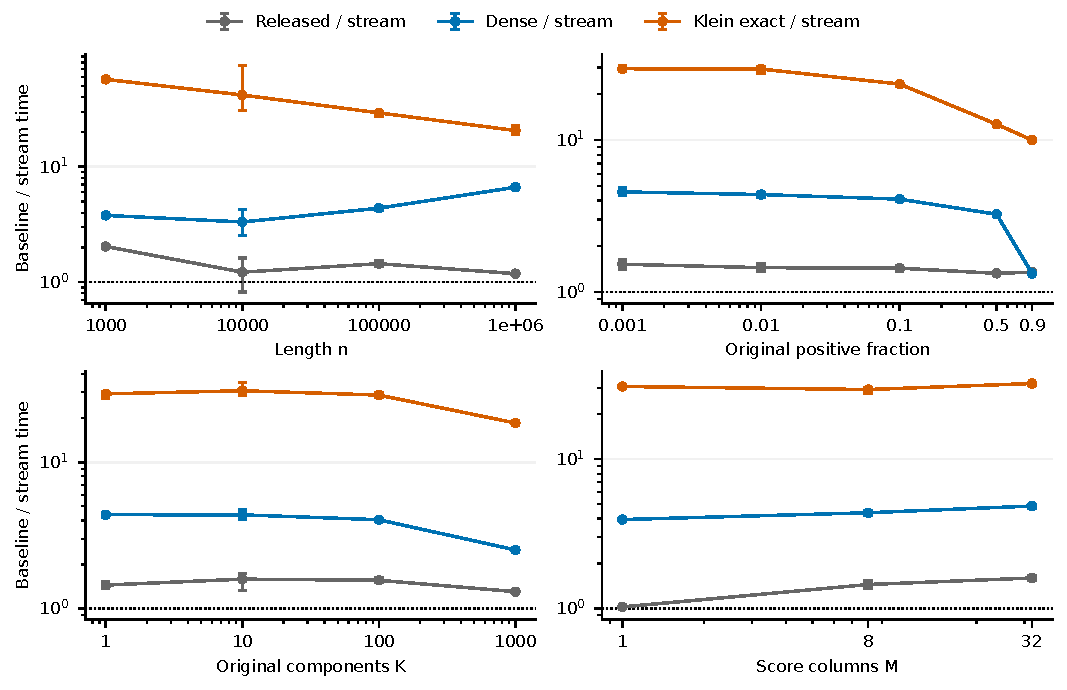
\includegraphics[width=.94\textwidth]{figures/pvldb_operating_range.pdf}
\caption{Controlled one-axis runtime conditions. Points and bars are paired
geometric time ratios and unadjusted 95\% trial intervals on four fixed-input
orders. Above one favors stream. All other parameters retain the common
anchor; the component axis also changes expanded support. These synthetic
mechanism checks supplement, rather than enlarge, the real-recording panel.}
\label{fig:operating-new}\end{figure*}

Post-timing diagnostics separately instrument the earlier active-prefix
algorithm. A dense independent reconstruction of interval ramps, complete
score ties and saturation verifies every visited-count array. At the
one-million-point random-score case, this algorithm visits 99.94\% of active
positions, explaining why recall saturation is not a general substitute for
support compression. At $K=1{,}000$, it visits 33.79\%; these counts do not
measure the different stream implementation's work or establish its timing.

\paragraph{Fresh execution on a second CPU.}
The one-command artifact was executed from a fresh checkout on a hosted Linux
runner with an AMD EPYC 7763 CPU, using the same source revisions, cohort,
detector parameters and balanced method orders. Raw data and public comparator
sources were downloaded and all scores generated anew. Both independent record
audits passed. At width 30, released/stream case ratios were 1.886, 1.580 and
1.340 for NAB, SMAP and SMD; the respective three-collection-adjusted 95\%
intervals were [1.732,2.043], [1.526,1.644] and [1.322,1.359]. All 73 case
medians favored stream. The exact Klein workflow ratios were 20.06, 20.28 and
16.17, while matched ROC+PR Benchopt/radix workflow ratios were 22.38, 30.40
and 42.55. Thus the direction of the main result survives a second CPU and a
fresh input-generation run. Hosted-runner load is uncontrolled: one NAB stream
workflow took 0.111 seconds against a 0.061-second median and is retained.
We report each host separately rather than pooling its timing repetitions.

Fresh detector scores differ across hosts, and so does the approximation result: 250 thresholds
change 13/73 winner sets on Linux, including three losses of at least 0.01,
versus 14/73 and four on the Mac. The difference is one SMAP case whose
approximate selected model changes, while its exact winner remains the same.
Its SVM exact VUS-PR changes from 0.3093 to 0.3329; we do not attribute this
observed difference to a particular numerical library operation without the
runner's generated arrays.
The 1,000-threshold counts remain three changed sets and zero losses of 0.01.
This sensitivity reinforces the distinction between a fixed-input numerical
comparison and a cross-platform detector-selection claim.

\paragraph{Process memory.}
A separately frozen resource study selects the real cases with largest length,
support fraction and component count, repeats the largest case's eight scores
four times for a declared $M=32$ stress case, and adds two synthetic density
cases at $n=500{,}000$, $M=8$. Three fresh processes per method record OS
lifetime peak RSS, including interpreter, libraries, inputs and tiny JIT warm-up.
This measures process resource use; subtracting two high-water marks does not
measure exact auxiliary space. On the real $M=8$ cases, stream peaks at
113.9--119.0 MiB; on the repeated $M=32$ case, 127.4 MiB versus released
125.5 MiB. The two synthetic cases expose the tradeoff more clearly
(Table~\ref{tab:memory-new}). At positive fraction 0.5, stream's peak is
225.0 MiB versus 175.2 MiB for released and 210.6 MiB for dense. Thus the
batch speed claim does not imply lowest peak memory. The largest numerical
PR discrepancy in this resource study is $1.67\cdot10^{-16}$; no timing
conclusion or real-data generalization is drawn from its synthetic inputs.

\section{Related work and novelty boundary}
The closest algorithmic work is the original VUS operator and its optimized
variants~\cite{paparrizos2022,boniol2025}. We preserve that operator. Temporal
weighting and proximity-aware PR are also established by
PATE~\cite{ghorbani2024pateproximityawaretimeseries}; we neither introduce those
ideas nor compare a different metric's runtime as if it returned VUS.
Sylligardos's efficient metric work~\cite{sylligardos2025} and current public
implementations motivate the semantic and source audit in Section~3.

TSB-AD~\cite{tsbad} studies large detector benchmarks and metric reliability;
TAB~\cite{qiu2025tabunifiedbenchmarkingtime} unifies benchmark data, methods and
evaluation. Our operator is a possible component of those systems, not a
replacement benchmark. TSB-AutoAD~\cite{liu2025autoad} compares selection,
ensembling and generation; RAMSAD~\cite{panourgias2026retrievaltrainingsimilaritysearchbased}
retrieves historical detector profiles for selection. We reduce the cost of
computing labeled profiles, without claiming superior unlabeled selection.
mTSBench~\cite{mtsbench} covers 344 multivariate series and 24 detectors, broader
than our targeted univariate operator workload. Analyses of foundation-model
pipelines~\cite{zhu2026} likewise address detection methodology rather than the
exhaustive scalar representation studied here.

Recent formal analysis of 37 metrics explicitly excludes score-based
volume-under-surface metrics from its formal scope~\cite{wagner2025formallyexploringtimeseriesanomaly}.
The resulting LARM/ALARM axioms do not establish our computational identity.
CCE~\cite{zhong2025cceconfidenceconsistencyevaluationtime} gives a different
linear-time metric; its speed is not an equal-output baseline. The metric
taxonomy~\cite{yang2026problemorientedtaxonomyevaluationmetrics} concerns
application requirements. Adversarial seed-shopping
analysis~\cite{lyu2026didactuallyfixit} varies reporting choices and compares
metrics, while our approximation experiment holds labels, score vectors and
the target fixed. None of these distinctions makes rank changes themselves a
new discovery. The narrow contribution is the exact event reduction, complete
global counts, dynamic integral correction and its measured implementation.

\section{Reproducibility and scope}
The artifact binds the public archive, each raw member, decoded observations,
labels, scores, method sources, trial orders and output records by SHA-256.
A single command creates a new isolated workspace, downloads pinned sources,
generates scores, executes both studies and reconstructs their numerical tables
as JSON (TeX rendering and manuscript compilation are separate):
\begin{quote}\small\ttfamily
python experiments/reproduce\_pvldb20261024.py\\
\hspace*{1em}--output /tmp/pvldb-replica
\end{quote}
It refuses an existing destination. Independent reconstruction imports no
metric producer and checks complete coverage, input/protocol/run bindings,
scalar values, winner sets, paired intervals and every principal-table field.
Corruption tests exercise changed intervals, fabricated summary entries,
replaced inputs, duplicate cases and false regret. Historical audit revisions
remain in the artifact. Fresh execution on the second CPU additionally checks
the full pipeline beyond reconstruction of recorded outputs.

The recorded environment is Python 3.12.4, NumPy 1.26.4, Numba 0.59.1,
pandas 3.0.1, scikit-learn 1.8.0 and SciPy 1.17.1. Detector scores can differ
across platforms even with these package pins; the cause of the observed
difference is undiagnosed. Each execution workspace retains its CPU, platform,
package versions and independently generated arrays. The archived Linux output
contains records and input hashes but omits the generated NPZ arrays. We do not
pool hosts into a single interval. Our CPU measurements do not establish GPU superiority;
the literature comparison is a bounded search of the stated sources.

The principal one-command execution covers the primary and public-comparator
supplement only. Long-recording/controlled, resource and minimal-Klein studies
have separate frozen protocols and commands in the artifact instructions.
The operating-range wrapper regenerates its inputs and checks its full design
before timing; its stages were executed in the recorded run, while the wrapper
itself has not received a second complete fresh execution. This boundary is
separate from the completed fresh primary/supplement run on Linux.

\paragraph{Limits.}
The principal evaluation uses short-to-moderate univariate series with sparse
anomalies and shared labels; the separate follow-up reaches 650,000 points on
real data and one million synthetically. Dense support and numerous fragments
are covered by controlled cases, not broad real-domain samples. Different
component-merging conventions, other VUS ramps, cold compilation and
training-dominated pipelines remain separate regimes. Whole-operator speed can
matter for repeated stored-profile queries even when the absolute savings on
one small collection are seconds. That use case must not be generalized to
end-to-end detector training. The mathematical statements use unit-cost metric
arithmetic; finite-precision experiments provide numerical parity, not an
all-input formal rounding proof. Batching uses more retained support state,
and its full public peak includes model-by-time validation/conversion arrays.

\section{Conclusion}
For the original dynamic VUS operator, inactive thresholds can be removed from
an exhaustive scalar computation only with complete global tie counts and the
appropriate ROC predecessor term. The resulting support-sensitive evaluator
preserves the target and permits shared-label evaluation. Three public
collections show numerical agreement and lower complete-call and workflow
cost than the measured exact comparators; the advantage also holds against the
measured sampled API. Modest incremental sharing gains, unfavorable prefix
cases, dependence and memory costs define the supported scope.

\bibliographystyle{ACM-Reference-Format}
\bibliography{sparse_vus_pvldb20261024_references}
\end{document}
